\chapter{Control }
\label{c5_DI2}
In this chapter we present the control architecture of the mobile robot.  
\section{Control Architecture and Hardware}


\begin{figure}
	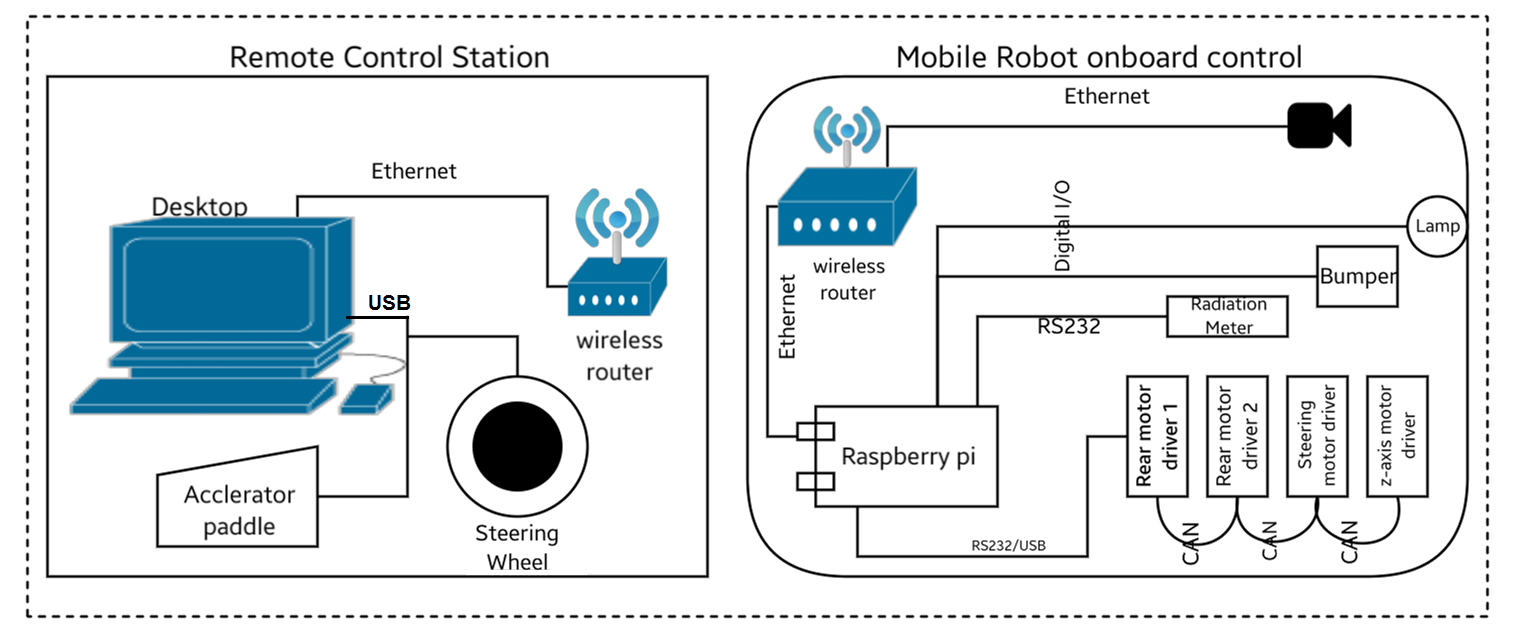
\includegraphics[width=\linewidth,keepaspectratio]{Chapter3/fig/controlblock}
	\captionof{figure}{Control Architecture Block Diagram }
	\label{fig:ControlBlockDiag} 
\end{figure} 
The mobile manipulator is planned to be teleoperated over a wireless network. The control block diagram and architecture are shown in Figure \ref{fig:ControlBlockDiag}. It has a remote control station which is the interface for the operator and a local controller on the mobile manipulator. They  communicate over a wifi network. The remote station send data packet every 50 millisecond to the mobile manipulator. The commanded velocity, the steer angle, the z position of the platform and the state of the detector and headlamps constitutes the data packet sent by the remote station. The on board control of the mobile robot replies with a data packet consisting of the $X$, $Y$ position and orientation of the robot, the current steer angle, angular velocities of each wheels, the z position of the top platform and bumper status.

\subsection{Local Onboard Controller}
The  on-board computer receives the command from the remote station and controls the robot hardware through Robot Operating System (ROS).
The computer is daisy chained to the four Maxon EPOS2 motor controllers/drivers. The communication between the onboard computer and the first Maxon controllers is over usb/RS232 interface using Maxon's proprietorial protocol~\cite{maxonrs232}. The first controller serves as CAN master for the rest of the controllers. The rear wheel motor drivers are configured in velocity servo loop. The steering and the z-axis motors drivers are configured in position control loop.  The camera mounted on the mobile robot  and Raspberry Pi  is connected over Ethernet via a wireless hub. 

\subsection{The Remote Control Station}   
The local station consists of a desktop computer running Windows XP. A Steering wheel and two foot switches are connected to the desktop. The steering wheel is used for turning  mobile robot. One of the two foot switch acts as an accelerator to set the mean velocity the other  is used to brake the vehicle.

The screen of the desktop displays the video streaming  from the mobile robot on board camera. A graphical user  interface (GUI) also displays the robot's parameters such as current steer angle, velocity of each rear wheel and the position of the z-axis. Buttons on the GUI operates the z-axis, head lamps, etc.

\begin{figure}[hbtp]
\centering
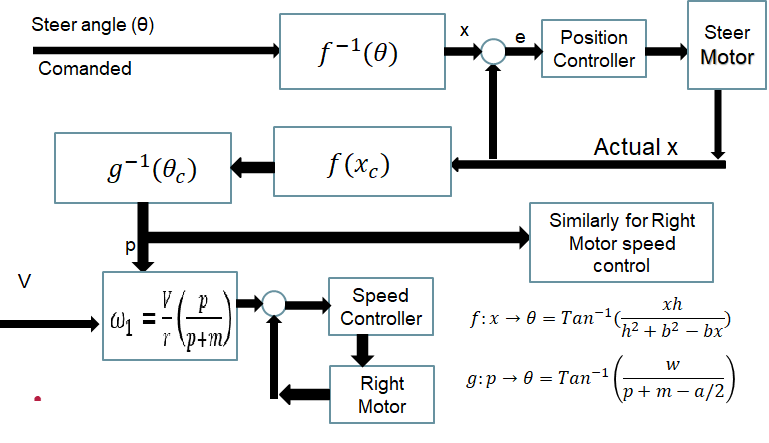
\includegraphics[scale=.5]{Chapter5/fig/BlkDigLocal.png}
\caption{Local Controller Block Digram}
\label{localBlock}
\end{figure}


\section{Admissible path}
\section{Trajectory Tacking}


\section{Summary}
In this chapter, 